%#####################################################################
\chapter{OpenFlowを用いたネットワークモデルの動作検証}
%#####################################################################

 本研究は,ネットワークシミュレータ上であるns-3上でOpenFlowを用いたネットワークモデルを構築し、シミュレーションを行い、ネットワークモデルが正常に動作するかを検証することが目的である。
ns-3では、シミュレーションによるトラフィックの流れをキャプチャすることが可能であるため、これを用いて作成したネットワークモデルの動作の検証を行った。
今回の動作検証の通信プロトコルはUDPとし、シミュレーション時間の前半に正方向の通信を、後半に逆方向の通信を行うようにした。

テストシナリオにおけるシミュレーションでは、パケット通信を可視化するPyVizでの表示と、PCAPファイル形式でパケットをダンプすることが可能となっている。
本章では、主にこの2つを用いて検証結果の評価を行った。

\section{ネットワークモデルの動作検証}

動作検証を行う際に、ホストの位置関係に関する2つのケース想定し、テストシナリオを作成した。

\begin{itemize}
	\item 送信元と送信先のコアスイッチの所属が違う場合
	\item 送信元と送信先のコアスイッチの所属が同じ場合
\end{itemize}

この2つのテストシナリオが正常に動作したならば、任意の2つのホスト間の通信は正常に動作したといえる。

\subsection{送信元と送信先のコアスイッチの所属が違う場合}

送信元と送信先のコアスイッチの所属が違う場合の通信として、図 \ref{fig:4-1}のような通信経路が一例として挙げられる。
この例に従い、C++を用いてテストシナリオを作成し、シミュレータ上で実行した。

\begin{figure}[tb]
\begin{center}
\scalebox{0.4}{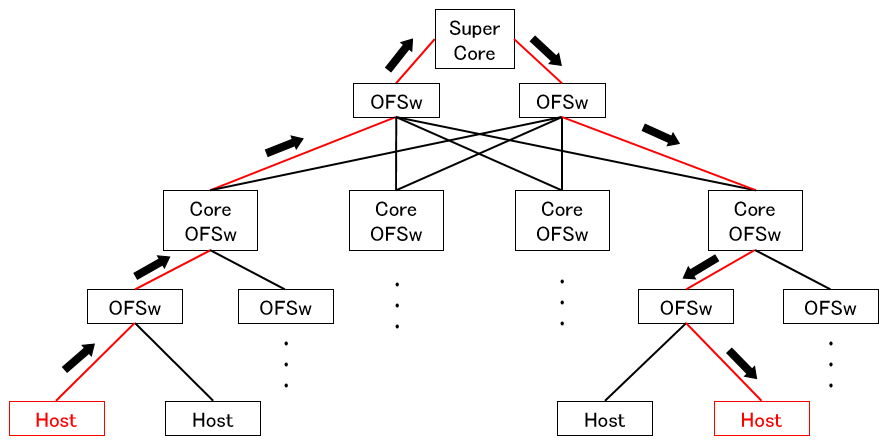
\includegraphics{./img/eps/4-1.eps}} 
\caption{送信元と送信先のコアスイッチの所属が違う場合の例}
\label{fig:4-1}
\end{center}
\end{figure}

\begin{figure}[tb]
\begin{center}
\begin{tabular}{c}

% 1
\begin{minipage}{0.4\hsize}
\begin{center}
\scalebox{0.3}{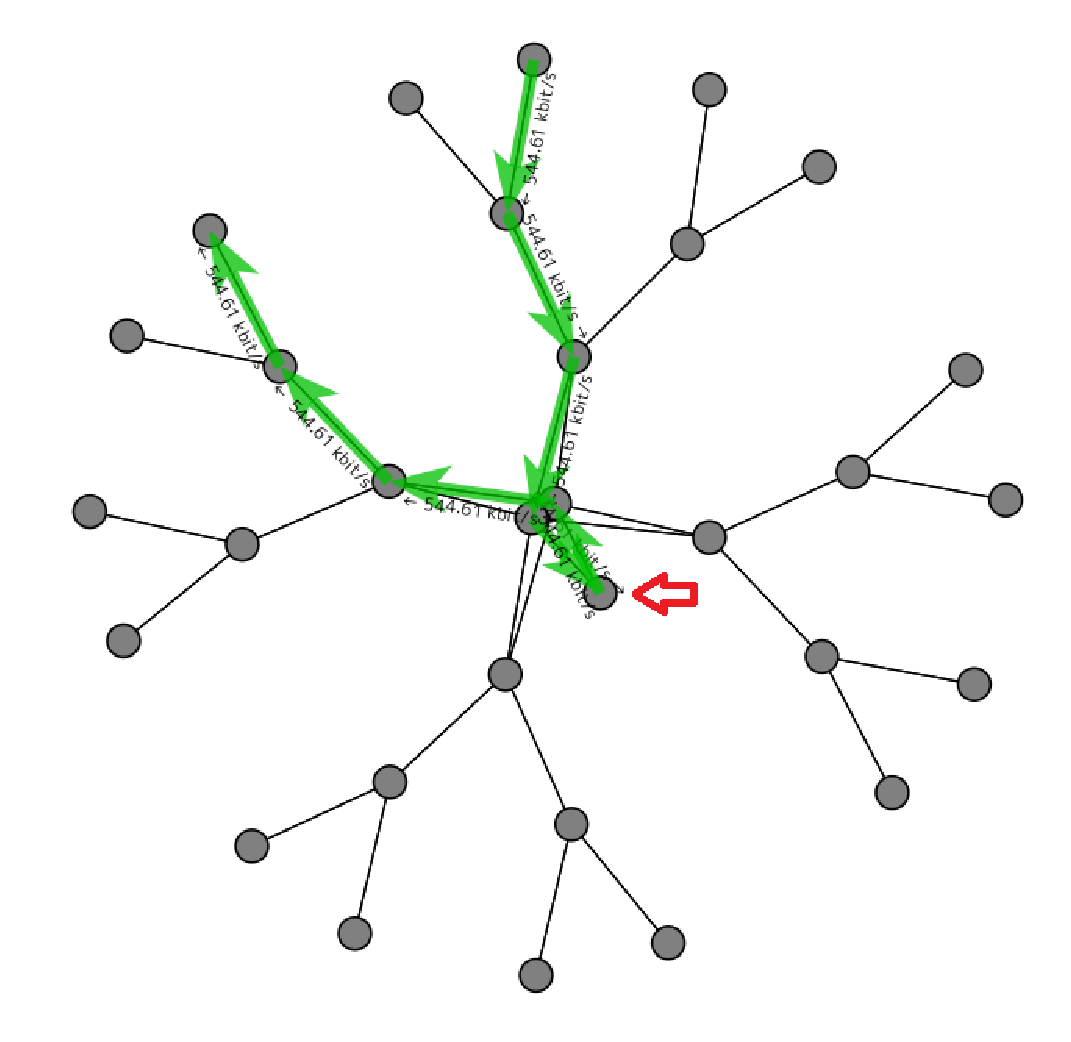
\includegraphics{./img/eps/4-2-1.eps}}
\hspace{1.6cm} [1]正方向の通信
\end{center}
\end{minipage}

% 2
\begin{minipage}{0.4\hsize}
\begin{center}
\scalebox{0.3}{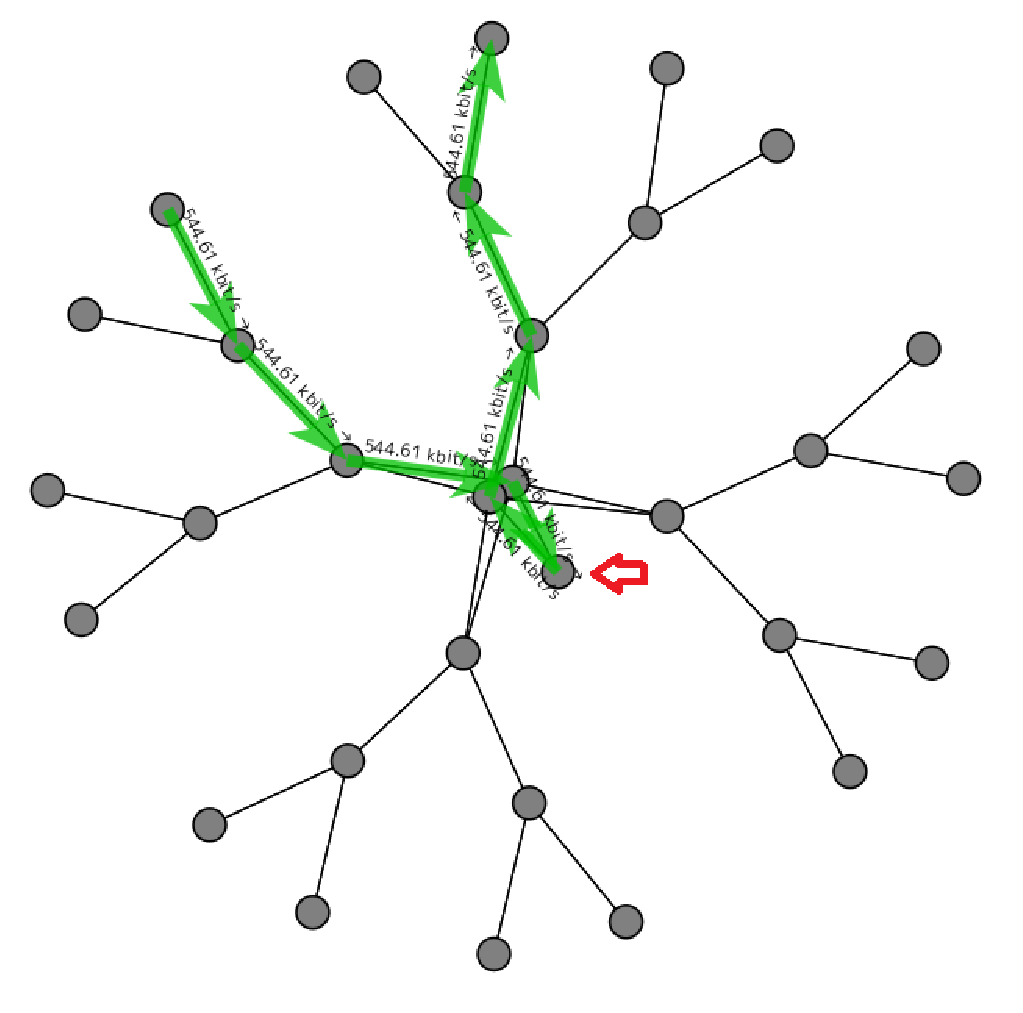
\includegraphics{./img/eps/4-2-2.eps}}
\hspace{1.6cm} [2]逆方向の通信
\end{center}
\end{minipage}

\end{tabular}
\caption{送信元と送信先のコアスイッチの所属が違う場合の結果}
\label{fig:4-2}
\end{center}
\end{figure}

図 \ref{fig:4-2}は、テストシナリオを用いてシミュレーションした際のパケット通信を可視化したものである。
図内の赤の矢印で示したノードがスーパーコアを想定したノードであり、正方向の通信、逆方向の通信ともにパケットが正常にこのノードを経由して通信を行っていることが分かる。
また、2つのホスト間の往復のパケットの経路が対称であることも確認できる。

\begin{figure}[tb]
	\begin{center}
		\begin{tabular}{c}
			
			% 1
			\begin{minipage}{0.4\hsize}
				\begin{center}
					\scalebox{0.3}{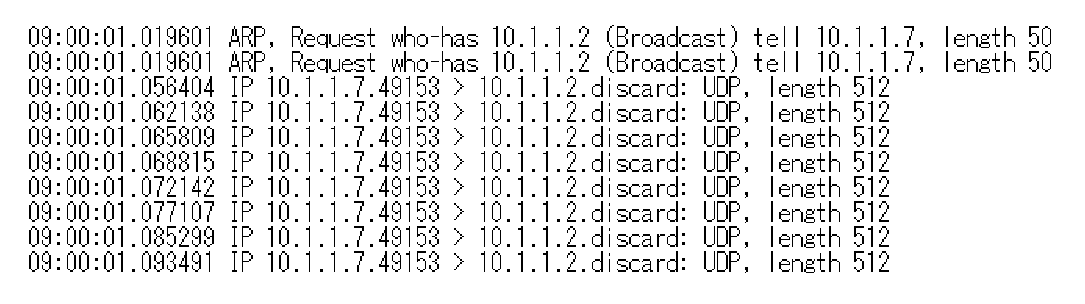
\includegraphics{./img/eps/4-3-1.eps}}
					\hspace{1.6cm} [1]正方向の通信
				\end{center}
			\end{minipage}
			
			% 2
			\begin{minipage}{0.4\hsize}
				\begin{center}
					\scalebox{0.3}{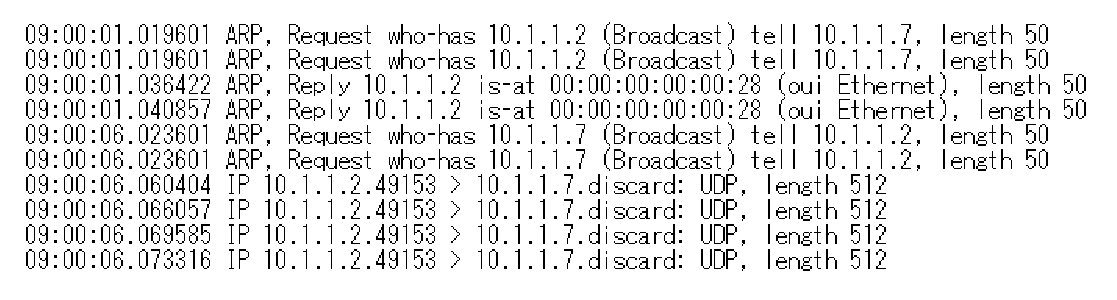
\includegraphics{./img/eps/4-3-2.eps}}
					\hspace{1.6cm} [2]逆方向の通信
				\end{center}
			\end{minipage}
			
		\end{tabular}
		\caption{送信元と送信先のコアスイッチの所属が違う場合のPCAPファイルの内容}
		\label{fig:4-3}
	\end{center}
\end{figure}

図 \ref{fig:4-3}は、スーパーコアのそれぞれの物理ポートでのパケット出力を示すトレースファイルから、最初の10パケットの通過を切り取ったものである。
今回のシミュレーションでは、正方向の通信は物理ポート0からの出力、逆方向の通信は物理ポート1からの出力であった。

トレースファイルによると、シミュレーションの前半にパケットを流した正方向の通信が例外なく物理ポート0から出力され、物理ポート1からは、ARPを除くと後半にパケットを流す逆方向の通信が出力されている。
つまり、MACアドレスの比較によるスーパーコアの入力ポート決定の方法も正常に動作しているといえる。

以上の内容からコアスイッチの所属が違う場合の通信は、すべてスーパーコアを通して通信されており、アルゴリズム通り正常に動作しているといえる。

\subsection{送信元と送信先のコアスイッチの所属が同じ場合}

送信元と送信先のコアスイッチの所属が同じ場合の通信として、図 \ref{fig:4-4}のような通信経路が一例として挙げられる。
この例に従い、C++を用いてテストシナリオを作成し、シミュレータ上で実行した。

\begin{figure}[tb]
	\begin{center}
		\scalebox{0.4}{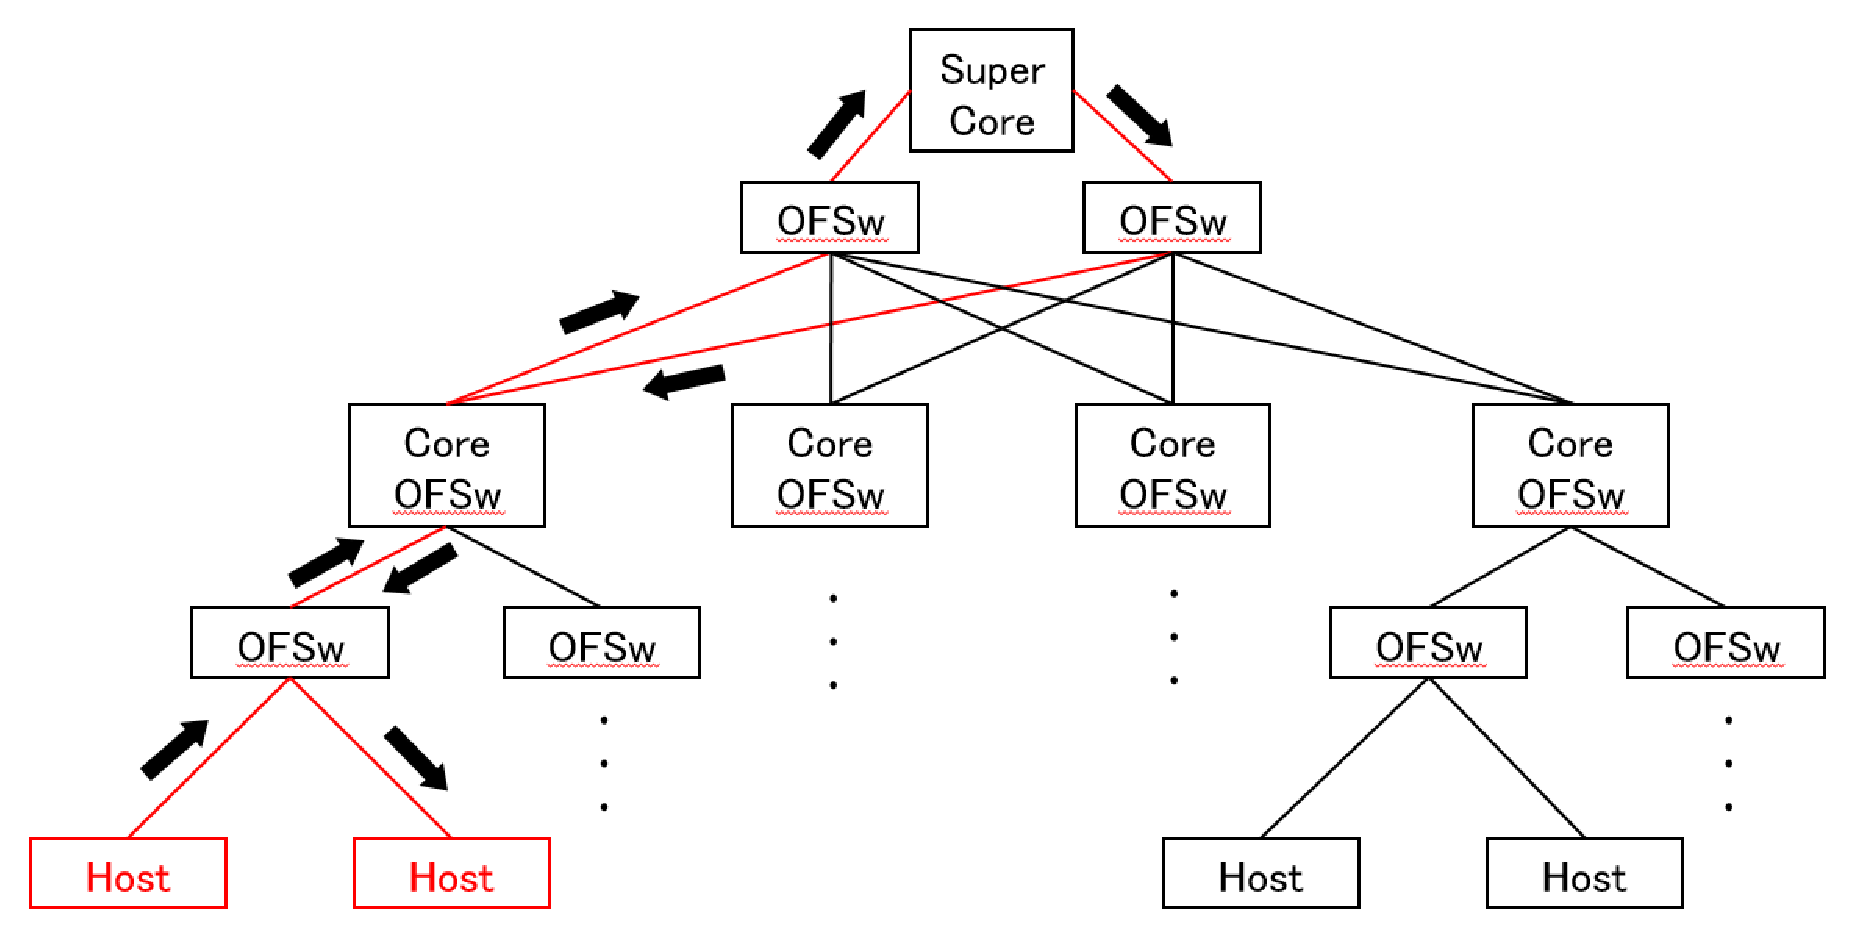
\includegraphics{./img/eps/4-4.eps}} 
		\caption{送信元と送信先のコアスイッチの所属が同じ場合の例}
		\label{fig:4-4}
	\end{center}
\end{figure}

\begin{figure}[tb]
	\begin{center}
		\begin{tabular}{c}
			
			% 1
			\begin{minipage}{0.4\hsize}
				\begin{center}
					\scalebox{0.3}{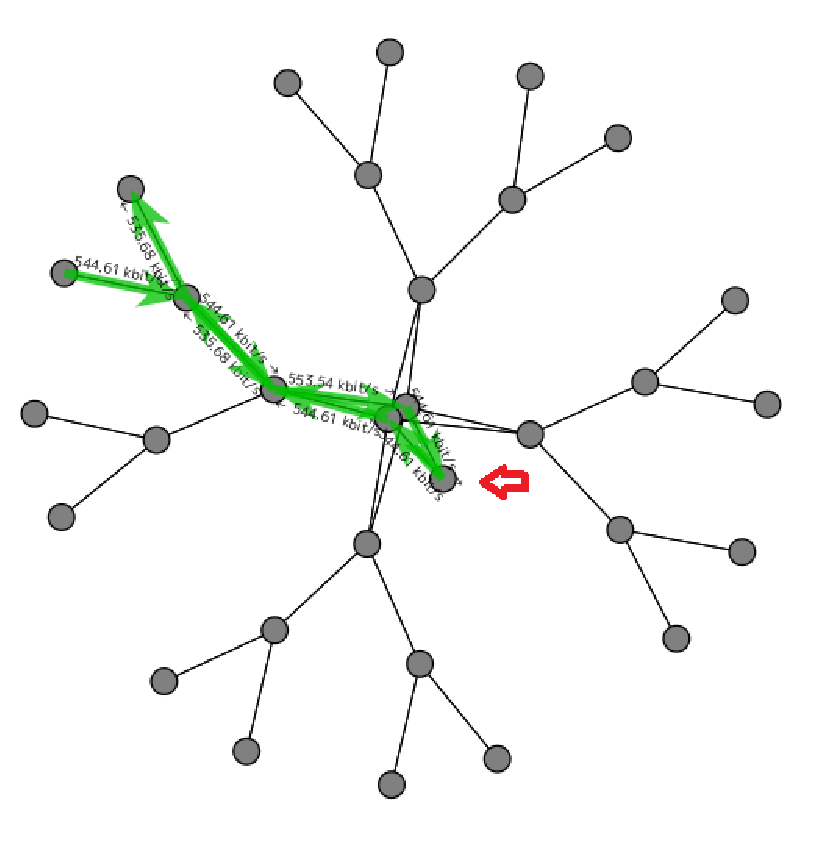
\includegraphics{./img/eps/4-5-1.eps}}
					\hspace{1.6cm} [1]正方向の通信
				\end{center}
			\end{minipage}
			
			% 2
			\begin{minipage}{0.4\hsize}
				\begin{center}
					\scalebox{0.3}{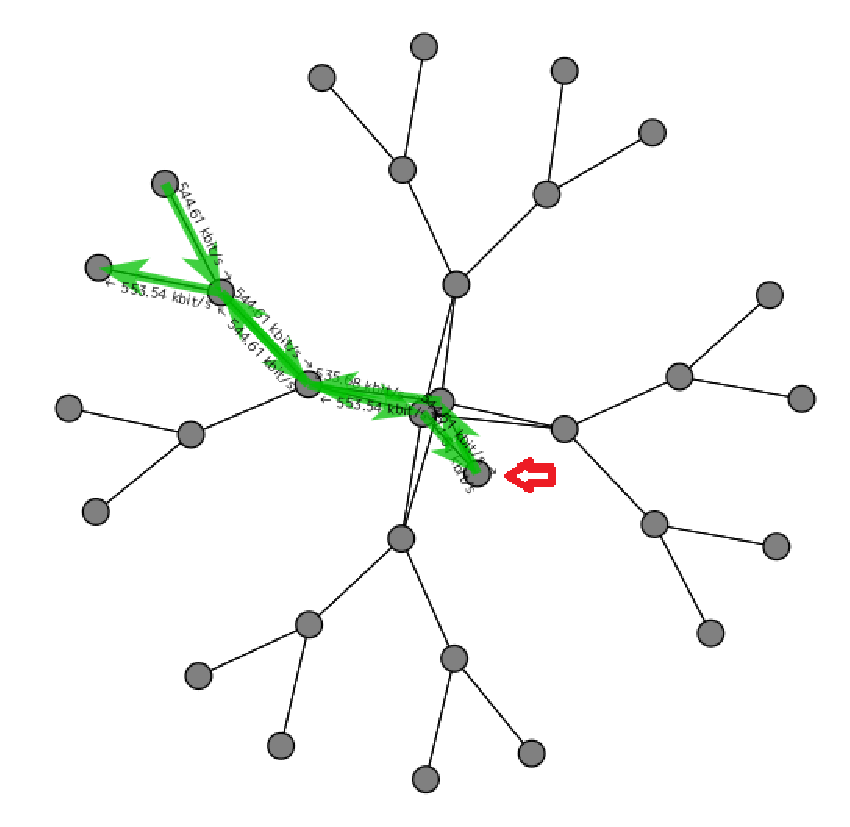
\includegraphics{./img/eps/4-5-2.eps}}
					\hspace{1.6cm} [2]逆方向の通信
				\end{center}
			\end{minipage}
			
		\end{tabular}
		\caption{送信元と送信先のコアスイッチの所属が同じ場合の結果}
		\label{fig:4-5}
	\end{center}
\end{figure}

図 \ref{fig:4-5}は、テストシナリオを用いてシミュレーションした際のパケット通信を可視化したものである。
図内の赤の矢印で示したノードがスーパーコアを想定したノードであり、正方向の通信、逆方向の通信ともにパケットが正常にこのノードを経由して通信を行っていることが分かった。
これにより、スイッチが自律的に最短経路によって経路選択をせずに、コントローラに従って動作していることも言える。
また、2つのホスト間の往復のパケットの経路が対称であることも確認できた。

\begin{figure}[tb]
	\begin{center}
		\begin{tabular}{c}
			
			% 1
			\begin{minipage}{0.4\hsize}
				\begin{center}
					\scalebox{0.3}{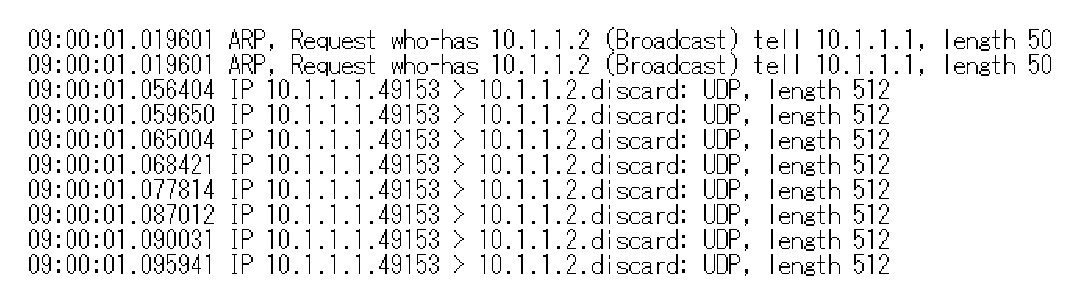
\includegraphics{./img/eps/4-6-1.eps}}
					\hspace{1.6cm} [1]正方向の通信
				\end{center}
			\end{minipage}
			
			% 2
			\begin{minipage}{0.4\hsize}
				\begin{center}
					\scalebox{0.3}{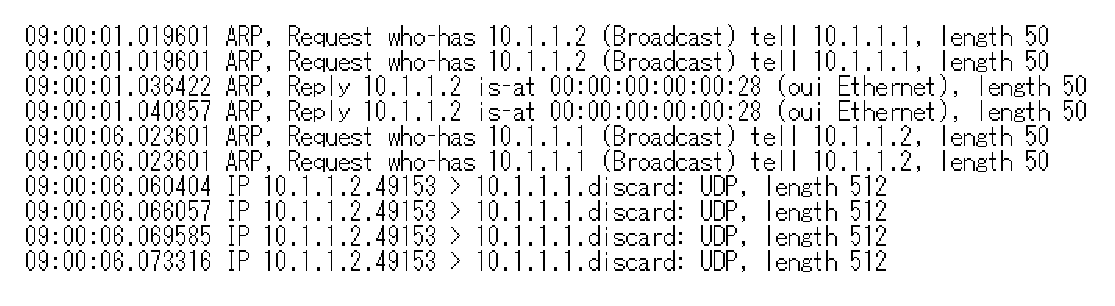
\includegraphics{./img/eps/4-6-2.eps}}
					\hspace{1.6cm} [2]逆方向の通信
				\end{center}
			\end{minipage}
			
		\end{tabular}
		\caption{送信元と送信先のコアスイッチの所属が同じ場合のPCAPファイルの内容}
		\label{fig:4-6}
	\end{center}
\end{figure}

図 \ref{fig:4-6}は、スーパーコアのそれぞれの物理ポートでのパケット出力を示すトレースファイルから、最初の10パケットの通過を切り取ったものである。
今回のシミュレーションでは、正方向の通信は物理ポート1からの出力、逆方向の通信は物理ポート0からの出力であった。

トレースファイルによると、シミュレーションの前半にパケットを流した正方向の通信が例外なく物理ポート1から出力され、物理ポート0からは、ARPを除くと後半にパケットを流す逆方向の通信が出力されていた。
つまり、MACアドレスの比較によるスーパーコアの入力ポート決定の方法も正常に動作しているといえる。

以上の内容からコアスイッチの所属が同じ場合の通信でも、すべてスーパーコアを通して通信されており、アルゴリズム通り正常に動作しているといえる。